\documentclass[a4paper]{article}

\usepackage[portuguese]{babel}
\usepackage[utf8]{inputenc}
\usepackage[T1]{fontenc}

\newcommand{\documentTitle}{Braitenberg Vehicles} %Macro definition
\newcommand{\documentAuthors}{João Rafael (2008111876) \and José Ribeiro (2008112181)} %Macro definition

\title{\documentTitle}
\author{\documentAuthors{}}

\usepackage{hyperref}
\hypersetup{
	pdftitle = \documentTitle
	,pdfauthor = \documentAuthors
	,pdfsubject = {Introduction to Artificial Inteligence Project \#1 Report}
	,pdfkeywords = {Artificial Inteligence Project} {Reactive Agents} {Braitenberg Vehicles}
	,pdfborder = {0 0 0}
}

\usepackage{subfig}
\usepackage{amsmath}
\usepackage{wrapfig}
\usepackage{array}
\usepackage{anysize}
\usepackage{lscape}
\usepackage[pdftex]{graphicx}

\marginsize{3.5cm}{3.5cm}{3cm}{3cm}

\makeatletter

\begin{document}
\renewcommand{\figurename}{Figure}
\maketitle
\cleardoublepage

\tableofcontents
\cleardoublepage

\setlength{\parindent}{1cm}
\setlength{\parskip}{0.3cm}

\section{Introduction}
% TODO

\cleardoublepage
\section{Breve Libraries}
\indent \indent Como referenciado na documentação da biblioteca Breve, o código Python fornecido é obtido através da compilação de código Steve.
Assim, esta biblioteca está pouco optimizada na medida em que não utiliza todas as potencialidades da linguagem.
Como tal, foram efectuadas algumas alterações no sentido de promover uma maior modularidade do código e flexibilidade.

\subsection{Constructors with parameters}
\indent \indent Uma das funcionalidades não utilizadas pelo Breve é a construção de objectos com parâmetros.
Desta forma, para criar um objecto é necessária uma chamada extra a uma função (\emph{init}).
Isto aumenta desnecessariamente o tamanho do código e dá azo a erros (utilização de objectos não inicializados).
Uma vez que todas as instâncias de objectos têm que ser criadas através da função \emph{createInstances} decidimos alterá-la de forma a transmitir os parâmetros utilizados durante a sua criação.
Consequentemente, é possível especificá-los directamente aquando da construção de veículos e cenários.

\subsection{Object distance}
\indent \indent Para implementar correctamente os sensores, é necessário calcular a distância entre dois objectos.
Para o cálculo desta distância as bibliotecas originais apenas têm em conta a distância euclidiana entre os centros.
No entanto esta aproximação não é suficiente quando os objectos têm dimensões elevadas.

\subsubsection{Point - Sphere}
\indent \indent Por definição, todos os pontos da superficie esférica estão à mesma distância do centro.
Desta forma a solução para o caso das esferas é apenas considerar a distância entre os centros e subtrair o raio da esfera.

\subsubsection{Point - Box}
\indent \indent Uma solução eficiente para este caso consiste em utilizar o algoritmo de Arvo como \\ descrito em  \footnote[1]{\url{http://www.gamasutra.com/view/feature/3383/simple_intersection_tests_for_games.php?page=4}}.
Este algoritmo necessita que a Box esteja alinhada com os eixos. Como este não é originalmente o caso, é necessário transformar as coordenadas do ponto no referencial original $O$ para o referencial da box $B$.
Esta transformação é obtida através do seguinte produto de matrizes:

\[
 	\begin{bmatrix}
		P_{x}' \\
		P_{y}' \\
		P_{z}' \\
		1 
	\end{bmatrix}
	=
	\begin{bmatrix}
		x_{x} & x_{y} & x_{z} & \vline & O_{x}	\\
		y_{x} & y_{y} & y_{z} & \vline & O_{y}	\\
		z_{x} & z_{y} & z_{z} & \vline & O_{z}	\\
		0 & 0 & 0 & \vline & 1 	\\
	\end{bmatrix}
	*
 	\begin{bmatrix}
		P_{x} \\
		P_{y} \\
		P_{z} \\
		1 
	\end{bmatrix}
\]

Onde $x, y, z$ são os versores do referencial $B$ em relação ao referencial $O$ e $O_{x}, O_{y}, O_{z}$ são as coordenadas da origem do referencial $O$ nas coordenadas do referencial $B$.

\cleardoublepage
\subsection{Activators}
\indent \indent Os veículos de Braitenberg, como definidos na literatura apenas permitem relacionar um sensor directamente com uma única roda.
Esta abordagem implica a replicação de sensores quando se pretende que estes tenham influências diferentes para cada roda.
Para evitar esta duplicação introduzimos o conceito de \emph{Activador}. 

Um \emph{Activador} é um bloco conceptual introduzido entre vários sensores e uma roda.
Este é responsável pelo cálculo das funções de activação de cada sensor e posterior agregação dos resultados, enviando depois o sinal correspondente para a roda. Desta forma, o veículo continua a ser um veículo de Braitenberg desde que a agregação dos resultados seja efectuada apenas com operações elementares (i.e: adição). 

%TODO

\subsection{Sensor rotation and initialization}
\indent \indent 

\subsection{Multibody collision handlers (Proxies, and Real's parents )}
\indent \indent A biblioteca do Breve apenas permite a detecção de colisões entre \emph{Shapes}. 
No entanto durante a execução do nosso projecto deparámo-nos com a necessidade de detectar a colisão entre dois objectos \emph{MultiBody}.
Para este efeito são colocados \emph{handlers} específicos para cada componente, que por sua vez efectuam \emph{event bubbling} para o objecto desejado.

\cleardoublepage
\section{Sensors}
\indent \indent Uma das partes que compõem um veículo de Braitenberg (e agentes reactivos na sua generalidade) são os sensores.
Estes comportam toda a entrada de dados fornecidos ao agente e podem apresentar diferentes complexidades.
Quanto mais realistas os sensores forem melhor é a qualidade máxima teórica dos agentes uma vez que estes possuem mais informação.
No entanto, mais complexidade necessita de mais poder computacional, tornando-se mais difícil de analisar (um fenómeno denominado por \emph{information overloading}).
Desta forma, é necessario efectuar \emph{trade-offs} de forma a encontrar um equilíbrio adequado.

\cleardoublepage
\subsection{Laser}

\begin{figure}[h]
	\vspace{-20pt}
	\begin{center}
		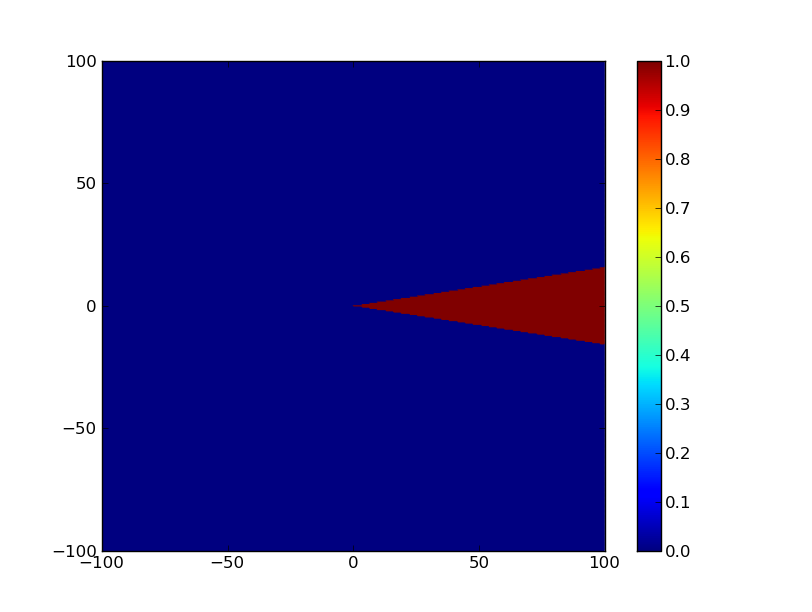
\includegraphics[width=0.6\textwidth]{graphs/sensors/laser.png}
	\end{center}
	\vspace{-20pt}
	\caption{Laser: $\alpha=\frac{\pi}{20}$}
\end{figure}

\indent Este sensor devolve simplesmente a existência ou não de objectos no seu ângulo, tendo assim um \emph{output} binário de -1 ou 1.
Assim, o \emph{output} do sensor é:
\[
	I = \left\{
		\begin{array}{lr}
			1 & : \text{caso exista um objecto no ângulo}\, \alpha \\
			-1 & : \text{caso contrário}
		\end{array}
		\right.
\]

onde $\alpha$ é a abertura do sensor ($rad$).


\cleardoublepage
\subsection{Distance}

\begin{figure}[h]
	\vspace{-20pt}
	\begin{center}
		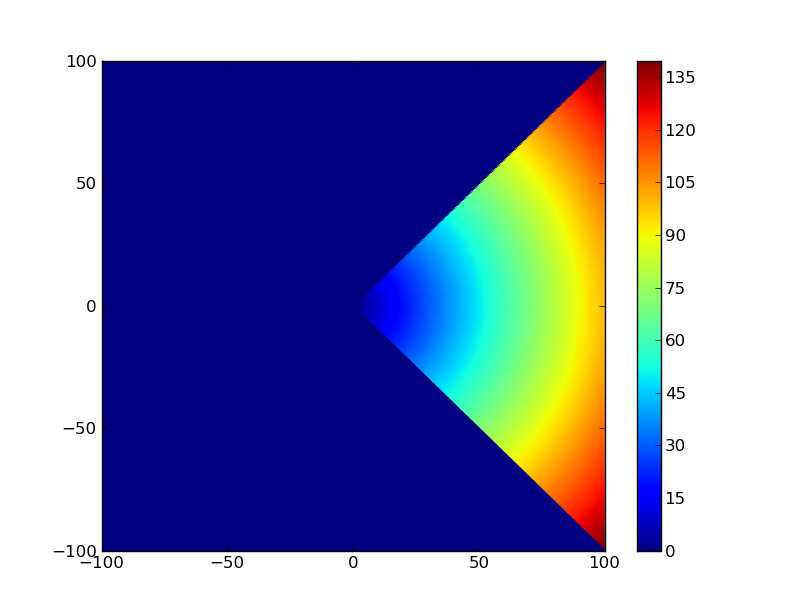
\includegraphics[width=0.6\textwidth]{graphs/sensors/distance.png}
	\end{center}
	\vspace{-20pt}
	\caption{Distance: $\alpha=\frac{\pi}{4}$}
\end{figure}

\indent Este sensor permite obter a mínima distância do sensor aos objectos dentro do seu ângulo de visão.
Assim, o \emph{output} do sensor é:
\[
	I = \min\{o_{d},\quad o \in objects \land o_{\alpha} < \alpha\}
\] 

onde $\alpha$ é a abertura do sensor ($rad$).

\cleardoublepage
\subsection{Proximity}
\begin{figure}[h]
	\vspace{-20pt}
	\begin{center}
		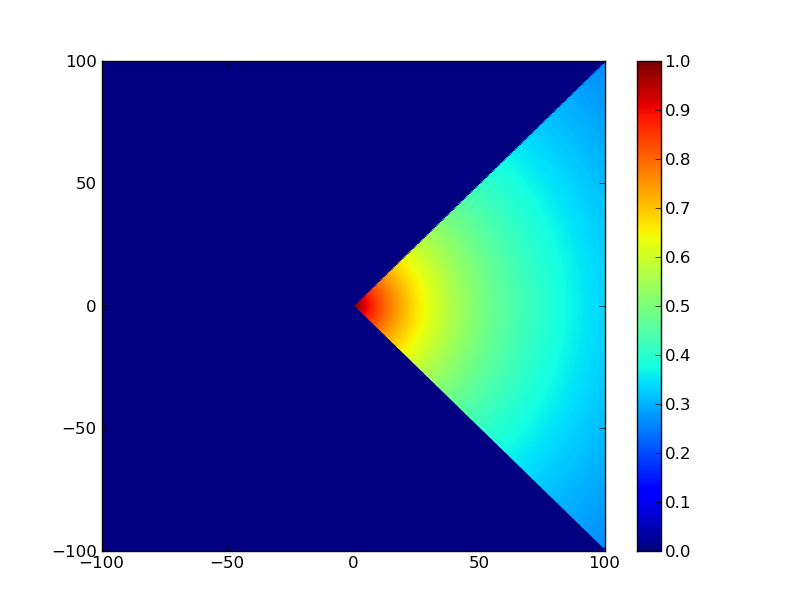
\includegraphics[width=0.6\textwidth]{graphs/sensors/proximity.png}
	\end{center}
	\vspace{-20pt}
	\caption{Proximity: \emph{half-distance}$=50$, $\alpha=\frac{\pi}{4}$}
\end{figure}

\indent O resultado deste sensor é inversamente proporcional à distância ao objecto mais próximo dentro do seu ângulo de visão.
O nível de decrescimento desta função é definido por \emph{half-distance} que indica a distância à qual se obtém o valor 0.5.
Desta forma a saida do sensor é:

\[
	I = \frac{1}{\frac{d_{min}}{d}+1},\quad d_{min} = \min\{o_{d},\quad o \in objects \land o_{\alpha} < \alpha\}
\]

onde $o_{d}$ é a distância do sensor ao objecto; $\alpha$ é o ângulo de visão do sensor e $d$ é a \emph{half-distance}.
Note-se que a função está deslocada uma unidade de forma a garantir valores no intervalo \[0..1\].

\cleardoublepage
\subsection{Smell}
\begin{figure}[h]
	\vspace{-20pt}
	\begin{center}
		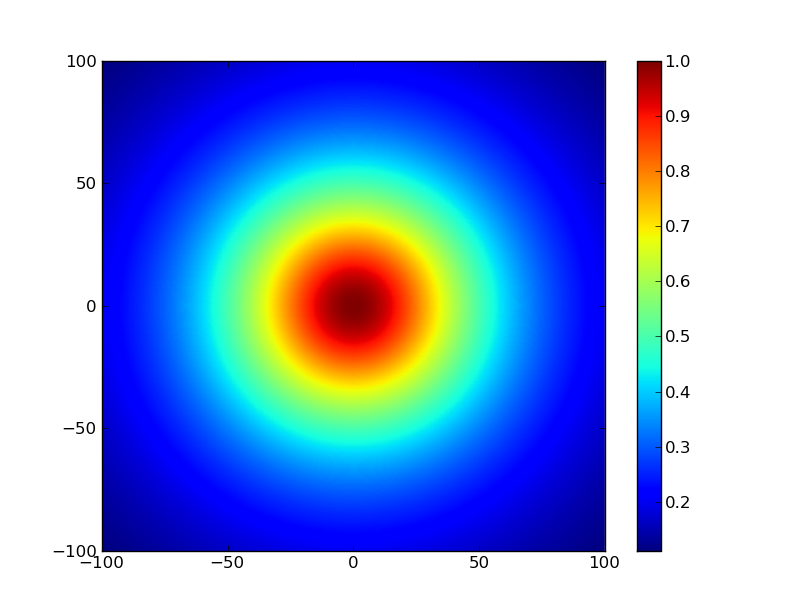
\includegraphics[width=0.6\textwidth]{graphs/sensors/smell.png}
	\end{center}
	\vspace{-20pt}
	\caption{Smell: \emph{half-distance}$=50$}
\end{figure}

\indent Este sensor indica a intensidade de cheiro captada. Esta intensidade é dada por um somatório das intensidades de todas as fontes de cheiro que privilegia as mais próximas do sensor. O factor de importância corresponde ao inverso do quadrado da distância do sensor a cada uma das fontes.
Assim, a intensidade deste sensor é:
\[
	I = \displaystyle\sum\limits_{s \in smell} \frac{s_{i}}{1 + (\frac{s_{d}}{d})^{2}}
\] 

onde $s_{i}$ e $s_{d}$ são a intensidade e a distância de cada fonte de cheiro, respectivamente; $d$ é a distância à qual uma fonte de cheiro com intensidade 1 situada em frente ao sensor produz uma saída no sensor de 0.5 (\emph{half-distance}).

Este sensor é omni-direcional, ao contrário de todos os outros sensores; como tal este não possui ângulo de abertura. 

\cleardoublepage
\subsection{Light}
\begin{figure}[h]
	\vspace{-20pt}
	\begin{center}
		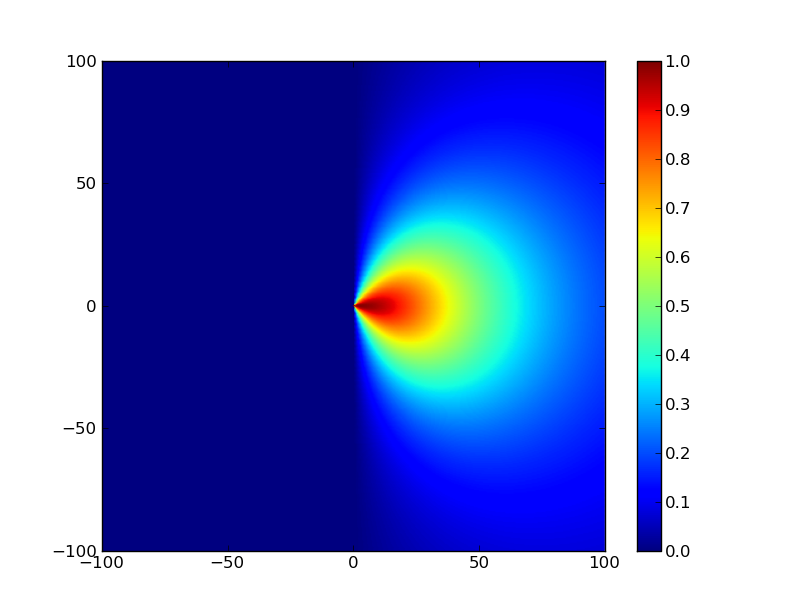
\includegraphics[width=0.6\textwidth]{graphs/sensors/light.png}
	\end{center}
	\vspace{-20pt}
	\caption{Light: \emph{half-distance}$=50$, $\alpha=\frac{\pi}{2}$}
\end{figure}

\indent Este sensor permite obter a intensidade de luz captada. Tal como no sensor de cheiro, a intensidade transmitida
é comulativa e inversamente proporcional ao quadrado da distância. No entanto, este sensor é direcionado (i.e. fontes
directamente à frente do sensor influenciam mais que os existentes na periferia). Assim, a intensidade total do sensor é:
\[
	I = \displaystyle\sum\limits_{l \in lights} \frac{l_{i}}{1 + (\frac{l_{d}}{d})^{2}*cos(\frac{2\pi}{\alpha}*l_{\alpha})}
\]

onde $l_{i}$, $l_{d}$, $l_{\alpha}$ são a intensidade, a distância e o ângulo de visão para cada luz, respectivamente;
$\alpha$ é a abertura do sensor ($rad$);
e $d$ é a distância à qual uma luz com intensidade 1 situada em frente ao sensor produz uma saída no sensor de 0.5.

\cleardoublepage
\subsection{Sound}
\begin{figure}[h]
	\vspace{-20pt}
	\begin{center}
		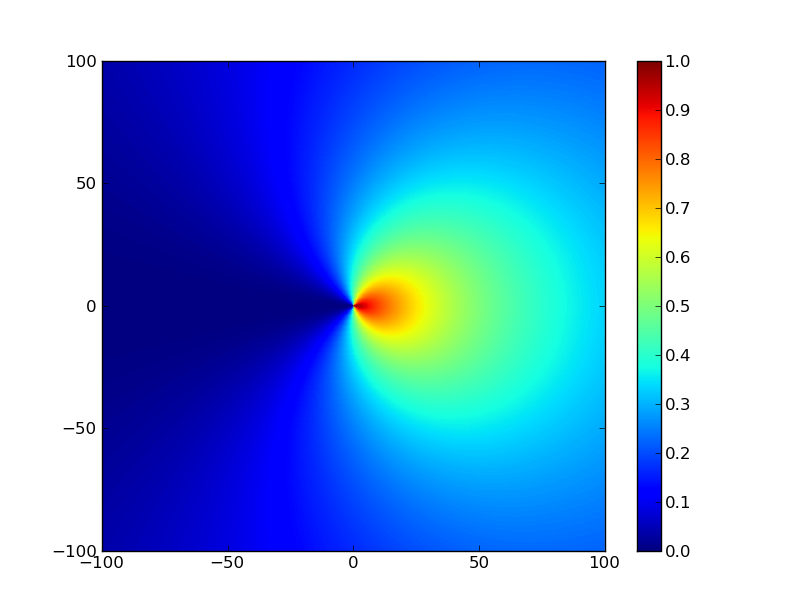
\includegraphics[width=0.6\textwidth]{graphs/sensors/cardioid.png}
	\end{center}
	\vspace{-20pt}
	\caption{Sound: \emph{half-distance}$=50$}
\end{figure}

\indent Este sensor indica a intensidade de som captado e pretende simular o
comportamento do ouvido humano. Desta forma, fontes de som em frente ao sensor têm mais impacto,
ainda que fontes atrás também o influenciem. Este comportamento foi bastante estudado e é aproximado pela função \emph{cardióide} definida em $\theta \in [0..2\pi]$:
\[
	cardioid(\theta) = \frac{1 + cos(\theta)}{2}
\]

\indent Extendendo esta função para 3 dimensões obtemos uma fórmula fechada para a superficie cardioidal
que utilizamos para construir o sensor de som cuja intensidade é
\[
	I = \displaystyle\sum\limits_{s \in sounds}\frac{1+cos(s_{\alpha})}{2}*\frac{s_{i}}{\frac{s_{d}}{d}+1}
\] 

onde $s_{i}$, $s_{d}$, $s_{\alpha}$ são a intensidade, a distância e o ângulo de fonte de som;
e $d$ a distância à qual uma uma fonte com intensidade 1 situada em frente ao sensor produz uma saída no sensor de 0.5.
Note-se que o resultado deste sensor é semelhante ao do sensor de luz quando $\alpha=\pi$,
mas decresce mais rapidamente quando o ângulo aumenta.

\cleardoublepage
\section{Vehicles}
%TODO

\subsection{Eight}
\begin{figure}[h]
	\centering

	\subfloat[Trail]{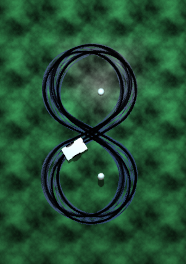
\includegraphics[width=0.2\textwidth]{trail/eight.png}}
	\subfloat[Left activator]{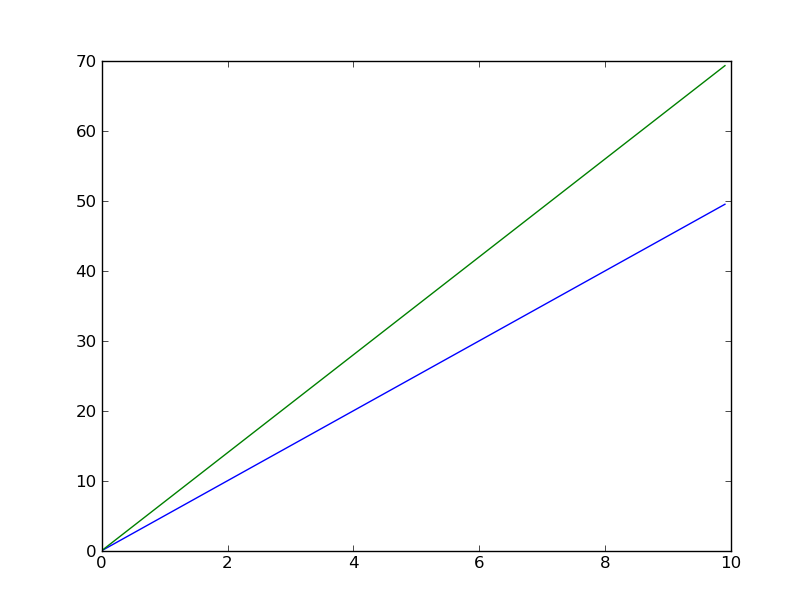
\includegraphics[width=0.4\textwidth]{graphs/activators/eight_l.png}}
	\subfloat[Right activator]{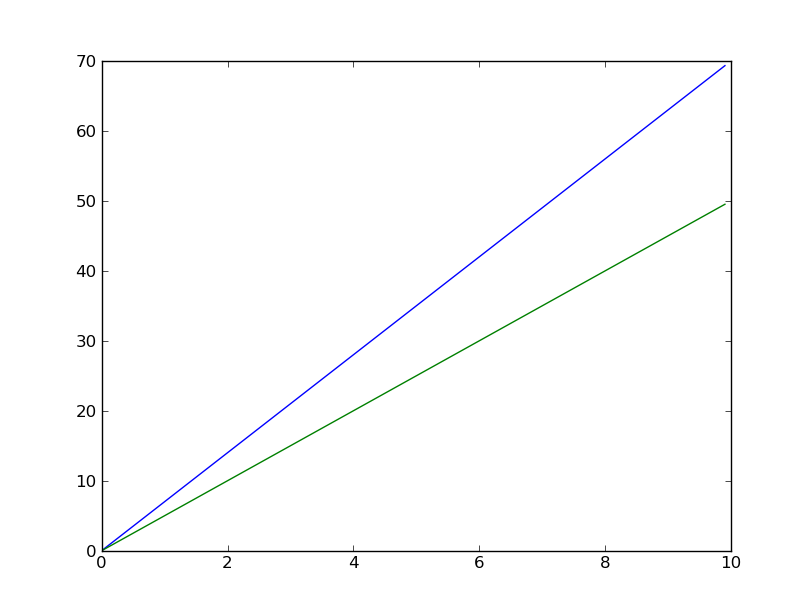
\includegraphics[width=0.4\textwidth]{graphs/activators/eight_r.png}}
	
	\caption{The eight vehicle}
\end{figure}


\cleardoublepage
\subsection{Ellipse}
\begin{figure}[h]
	\centering
	\subfloat[Trail]{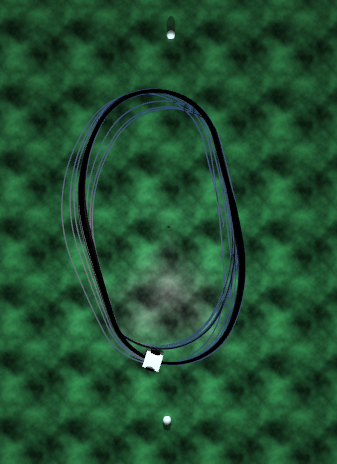
\includegraphics[width=0.2\textwidth]{trail/ellipse.png}}
	\subfloat[Left activator]{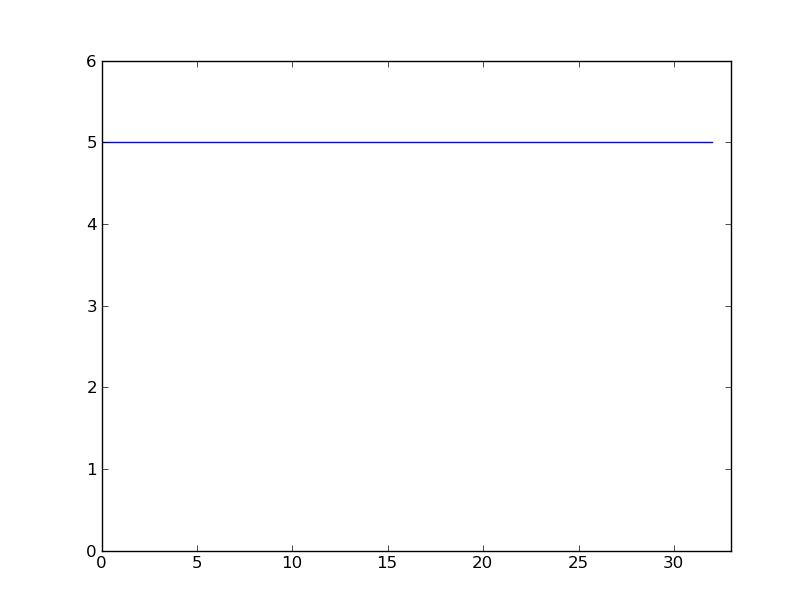
\includegraphics[width=0.4\textwidth]{graphs/activators/ellipse_l.png}}
	\subfloat[Right activator]{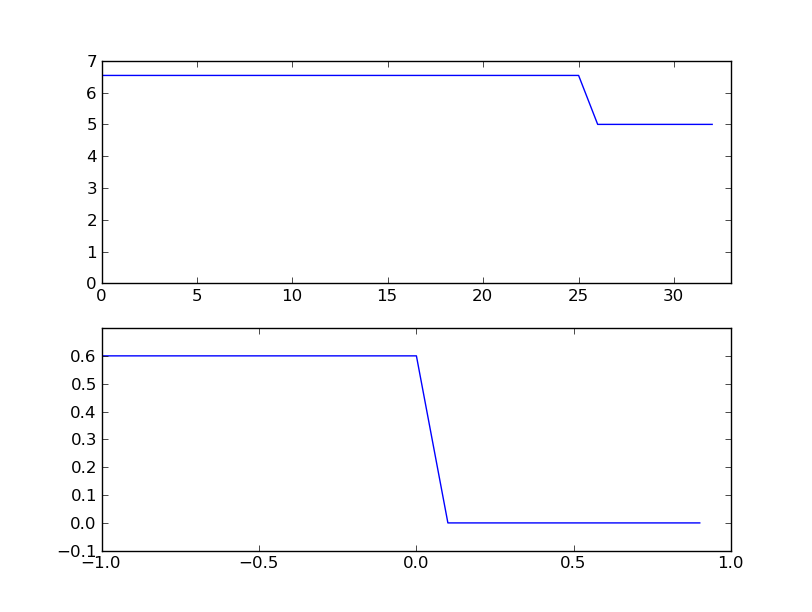
\includegraphics[width=0.4\textwidth]{graphs/activators/ellipse_r.png}}
	
	\caption{The ellipse vehicle}
\end{figure}

\cleardoublepage
\subsection{Aggressor/Explorer}
\begin{figure}[h]
	\centering
	\subfloat[Left activator]{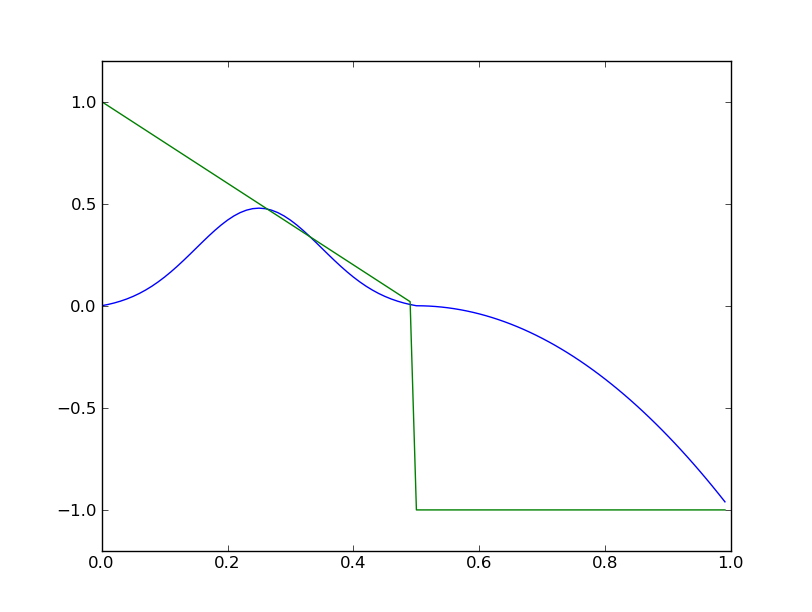
\includegraphics[width=0.4\textwidth]{graphs/activators/aggr_expl_l.png}}
	\subfloat[Right activator]{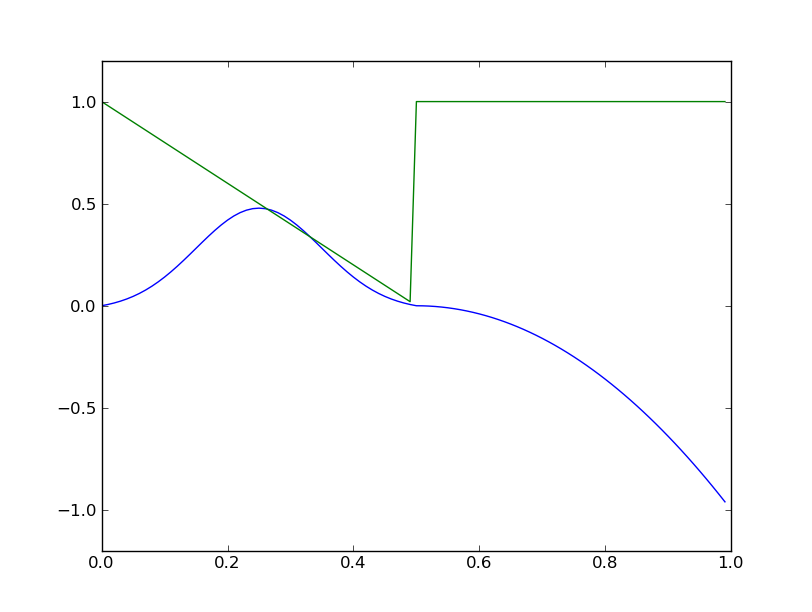
\includegraphics[width=0.4\textwidth]{graphs/activators/aggr_expl_r.png}}
	
	\caption{The Aggressor/Explorer vehicle}
\end{figure}

Este veículo vive num mundo com dois tipos de objectos: luzes e obstáculos.
O seu objectivo é explorá-lo, desviando-se dos obstáculos e explorando as luzes, i.e.,
aproxima-se delas como se estivesse curioso, após o qual perde o interesse seguindo à procura de novas.

Para se observar este comportamento a função de activação em relação aos obstáculos é decrescente até 0.5 (momento em que atinge \emph{half-distance}).
Após este valor assume-se que o veículo está preso e precisa de voltar para trás (rodar), pelo que se aplica uma intensidade simétrica em cada roda.

Quanto às luzes a função de activação cresce até 0.25 (o veículo vê uma luz e tenta aproximar-se rapidamente) e decresce até 0.5 (abranda para poder observar).
Após este valor a função assume valores cada vez menores (e negativos), de forma a afastar-se (uma vez que este sensor se encontra ligado de forma cruzada).

\cleardoublepage
\subsection{Braitenberg 3c}
\begin{figure}[h]
	\centering
	\subfloat[Left activator]{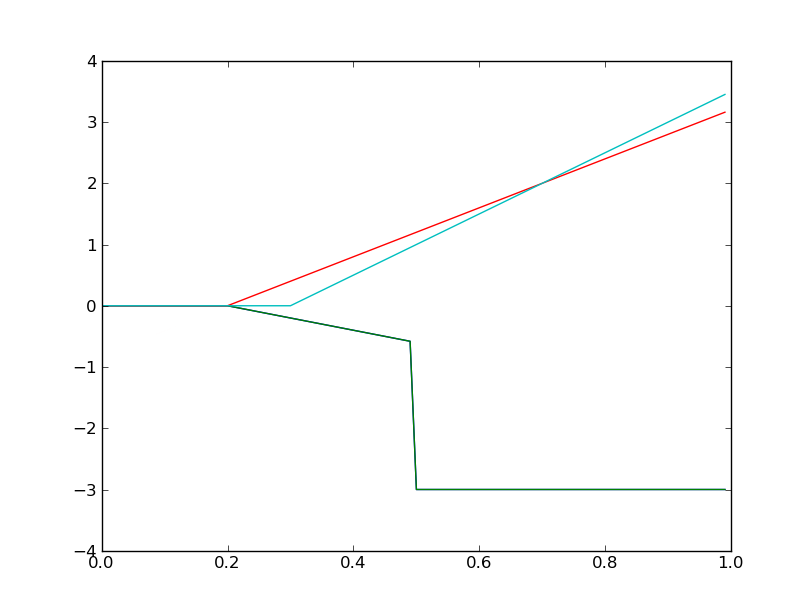
\includegraphics[width=0.5\textwidth]{graphs/activators/3c_l.png}}
	\subfloat[Right activator]{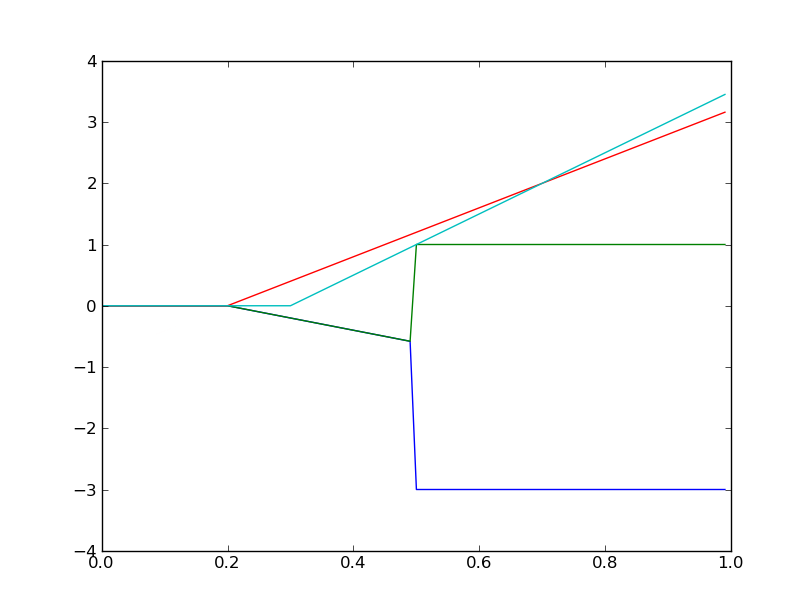
\includegraphics[width=0.5\textwidth]{graphs/activators/3c_r.png}}
	
	\caption{The Braitenberg 3c vehicle}
\end{figure}
Apesar do veículo sugerido possuir na mesma 4 sensores, este não é o Braitenberg 3c tal como definido por Valentino na sua obra.
No entanto, da mesma forma que Braitenberg avaliou a psicologia sintética dos seus veículos (regidos apenas por reações),
podemos avaliá-lo sob a mesma perspectiva.

Este veículo apresenta um comportamento bastante complexo. Pretende explorar todo o ambiente (luzes e obstáculos), gosta de 
correr no meio de flores (fontes de cheiro) e tem medo dos seus predadores (fontes de som). 

Para garantir este comportamento foram utilizadas funções de corte inibidoras quando as intensidades do sensores são pequenas.
Este corte evita que a soma dos vários comportamentos se acumule e o veículo se comporte de forma errática.
No entanto, quando 2 ou mais sensores apresentam intensidades superiores ao corte o comportamento corresponde à sua sobreposição.
Neste caso o resultado final pode não ser o melhor.


\cleardoublepage
\section{Project - Braitenberg Population}
\begin{figure}[h]
	\centering
	\subfloat[Group behaviour]{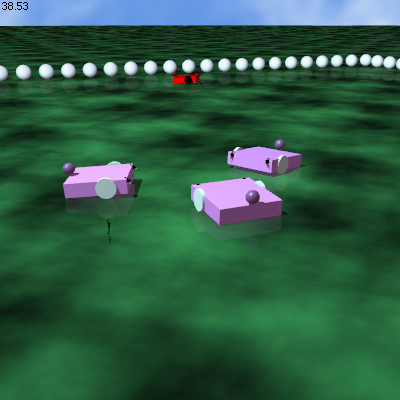
\includegraphics[width=0.3\textwidth]{screenshots/gossiping.png}}
	\hspace{5px}
	\subfloat[Sexual Opportunism]{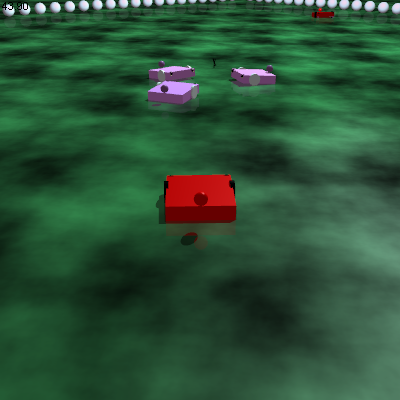
\includegraphics[width=0.3\textwidth]{screenshots/opportunism.png}}
	\hspace{5px}
	\subfloat[Protective instinct]{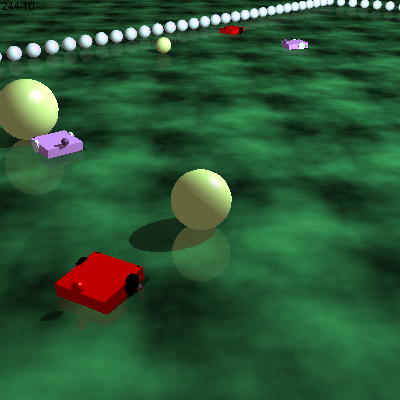
\includegraphics[width=0.3\textwidth]{screenshots/protective.png}}

	\caption{Braitenberg Population}
\end{figure}

% Both
Instinto protector

% Females
Instinto Maternal
Aptidao social
Comportamento de grupo 

% Males
Comportamento individual
Comportamento sexual

\end{document}
